\section{Dimuon mass and lifetime dimensions}
\label{sec:mass-lifetime}

As we have seen in the previous chapter,
the measurement of the \lth polarization parameter of 
the prompt (or non-prompt) \jpsi (or \psip) mesons 
is made by fitting the ratio between the corresponding measured and simulated 
two-dimensional $(\abscosth,\pt)$ distributions.
While the MC distribution is already the needed one (only the signal is simulated),
the measured distribution needs to be computed by subtracting 
the relevant background terms from the directly measured distribution 
(Eqs.~\ref{eq:bkgSub_psi_PR} and~\ref{eq:bkgSub_psi_NP}).

We will report in this chapter our studies of the mass and lifetime dimensions, 
leading to the evaluation of the needed 2D $(\abscosth,\pt)$ distributions
and of the corresponding fractions, as functions of \pt.

%%%%%%%%%%%%%%%%%%%%%%%%%%%%%%%%%%%%%%%%
\subsection{The dimuon mass distribution}
\label{sec:mass}

For simplicity, the analysis is only described for the \jpsi case,
but it applies in an analogous way for the \psip case.

The dimuon mass distribution is described by the superposition of
a double Crystal-Ball function plus a Gaussian function 
to describe the \jpsi signal line shape ($L_{\psi}$)
and a decreasing exponential function 
to describe the underlying mass continuum background ($L_{\rm Bg})$:

\begin{equation}
L_{\psi} = f_{CB_1}\cdot g_{CB_1}(m) + (1-f_{CB_1}-f_G)\cdot g_{CB_2}(m) + f_G\cdot g_{G}(m)
\end{equation}


\begin{equation}
L_{\rm Bg} = N_{\rm Bg} \; \exp(-m/t_{\rm Bg})
\end{equation}


The fraction $f_{\rm Bg}$ of events in the Peak region
corresponding to ``continuum muon pairs"
is computed by integrating the $L_{\rm Bg}$ function
in the 3.0--3.2~GeV mass window 
and then dividing the result by the total number of events
counted in that mass range.

The two CB functions have common means, $\mu_m$, and tail parameters, $n$ and $\alpha$,
and independent widths, $\sigma_{CB_1}$ and $\sigma_{CB_2}$.
The Gaussian function has the same mean, $\mu_m$, 
and an independent width, $\sigma_{G}$.

Independently fitting the dimuon mass distributions in each of the 19 \pt bins 
would naturally lead to results affected by random statistical fluctuations,
especially if all shape parameters would be left free.
We know that some of the parameters are (anti-)correlated and it is not reasonable 
to leave them all free in the fit 
(that is the case, in particular, of the $n$ and $\alpha$ tail parameters).
We also know that the shape parameters of the $L_{\psi}$ and $L_{\rm Bg}$ functions
must change with \pt in a smooth way.

After a series of preliminary studies of the (simulated and measured) dimuon mass distributions,
we converged on a fit model that is able to faithfully describe the data 
with a relatively small number of free shape parameters,
determined from the \emph{simultaneous} fit of the 19 mass distributions,
either as constants or as linear functions of \pt.
We think that this relatively simple model represents a good balance 
between having too many free parameters 
(leading to under-constrained fits and results affected by random statistical fluctuations)
and having too many arbitrarily-selected constraints
(possibly leading to results biased by our specific assumptions).

\vfill\newpage

The fit model used for the \jpsi analysis is constrained as follows:
\begin{itemize}
\item $\mu_m$, $f_{CB_1}$ and $\alpha$ are independent of \pt;
\item $\sigma_{CB_1}$, $\sigma_{CB_2}$ and $\sigma_{G}$ 
are linear functions of \pt with a common slope;
\item $f_G = 3.5\%$ and $n = 2.5$.
\end{itemize}

The only difference in the \psip fit model is that we set $f_G = 2.5\%$
instead of 3.5\%. We have seen, however, that this very small term could even 
be simply neglected, as it has no effect at all on the results of the analysis
(we only include it to avoid non-negligible pulls on the right side tail of the \jpsi).

The inverse slopes of the mass continuum exponential function, $t_{\rm Bg}$,
are left free in all \pt bins. 
This is the most important shape parameter of the dimuon mass fits,
for the purpose of our analysis, given that all we need from these fits is
the fraction $f_{\rm Bg}$, versus \pt.

The fitted $t_{\rm Bg}$ values are shown in Fig.~\ref{fig:tbkg-psi}, 
for the \jpsi (left) and \psip (right) analyses.

\begin{figure}[h]
\centering
\includegraphics[width=0.48\textwidth]{Figures/chapter4/par_tbkg-jpsi.pdf}
\includegraphics[width=0.48\textwidth]{Figures/chapter4/par_tbkg-psip.pdf}
\caption{Fitted $t_{\rm Bg}$ versus \pt, for the \jpsi (left) and \psip (right) analyses.}
\label{fig:tbkg-psi}
\end{figure}

\vfill\newpage

The measured mass distributions are well described by the fit model;
there are no systematic trends in the pull distributions. 
Figure~\ref{fig:mass-fits-psi} illustrates the fit quality in the \jpsi case, 
for two typical \pt bins.

\begin{figure}[h]
\centering
\includegraphics[width=0.45\textwidth]{Figures/chapter4/Mfit_pt4.pdf}
\includegraphics[width=0.45\textwidth]{Figures/chapter4/Mfit_pt14.pdf}\\
\includegraphics[width=0.45\textwidth]{Figures/chapter4/Mpulls_pt4.pdf}
\includegraphics[width=0.45\textwidth]{Figures/chapter4/Mpulls_pt14.pdf}
\caption{Fitted \jpsi mass distributions for two \pt bins (top) 
and corresponding pull distributions (bottom).}
\label{fig:mass-fits-psi}
\end{figure}

\vfill\newpage

Figures~\ref{fig:mass-fits-psip-PR} and~\ref{fig:mass-fits-psip-NP} show
the corresponding plots for the \psip, respectively for the prompt and non-prompt cases.

\begin{figure}[hb!]
\centering
\includegraphics[width=0.33\textwidth]{Figures/chapter4/Pfit_pt2.pdf}
\includegraphics[width=0.33\textwidth]{Figures/chapter4/Pfit_pt5.pdf}\\
\includegraphics[width=0.33\textwidth]{Figures/chapter4/Ppulls_pt2.pdf}
\includegraphics[width=0.33\textwidth]{Figures/chapter4/Ppulls_pt5.pdf}
\caption{Fitted prompt \psip mass distributions for two \pt bins (top) 
and corresponding pull distributions (bottom).}
\label{fig:mass-fits-psip-PR}
%\end{figure}
%
%\begin{figure}[h]
\centering
\includegraphics[width=0.3\textwidth]{Figures/chapter4/Nfit_pt2.pdf}
\includegraphics[width=0.3\textwidth]{Figures/chapter4/Nfit_pt5.pdf}\\
\includegraphics[width=0.3\textwidth]{Figures/chapter4/Npulls_pt2.pdf}
\includegraphics[width=0.3\textwidth]{Figures/chapter4/Npulls_pt5.pdf}
\caption{Fitted non-prompt \psip mass distributions for two \pt bins (top) 
and corresponding pull distributions (bottom).}
\label{fig:mass-fits-psip-NP}
\end{figure}

\vfill\newpage

As mentioned before, 
the fraction of mass continuum muon pairs in the Peak window, $f_{\rm Bg}$, 
is evaluated (in each \pt bin) by integrating the fitted background function 
in that window and dividing the result by the total number of events in that window.
The results are shown in Fig.~\ref{fig:fBg}, for the prompt and non-prompt
\jpsi and \psip analyses.

\begin{figure}[h]
\centering
\includegraphics[width=0.4\textwidth]{Figures/chapter4/fBG_unc_jpsi.pdf}
\includegraphics[width=0.4\textwidth]{Figures/chapter4/fBGNP_unc_jpsi.pdf}
\includegraphics[width=0.4\textwidth]{Figures/chapter4/fBG_unc_psip.pdf}
\includegraphics[width=0.4\textwidth]{Figures/chapter4/fBGNP_unc_psip.pdf}
\caption{Measured $f_{\rm Bg}$ fractions vs.\ \pt, 
for the prompt (left) and non-prompt (right) \jpsi (top) and \psip (bottom) analyses.}
\label{fig:fBg}
\end{figure}

\vfill\newpage

%%%%%%%%%%%%%%%%%%%%%%%%%%%%%%%%%%%%%%%%
\subsection{The dimuon lifetime distribution}
\label{sec:lifetime}

The dimuon lifetime distribution, 
in the window from $-50$ to $+500\,\mu$m,
is described by the superposition of two terms: 
the prompt and non-prompt contributions.

The PR term is, effectively, the lifetime resolution function.
Given that we are considering a sample of events integrated over rapidity,
and knowing that the lifetime resolution is not independent of rapidity,
it is reasonable to assume that the resolution function should be the convolution
of many Gaussian functions.
In practice, the sum of only two Gaussian functions already provides a 
sufficiently-good description of the data, at least for our purposes:

\begin{equation}
L_{\rm PR} \equiv L_{\rm res} = 
f_{G_1} \times G_{1}(c\tau|\mu_{c\tau}, \sigma_{G_1})
+(1-f_{G_1}) \times G_{2}(c\tau|\mu_{c\tau}, \sigma_{G_2}) \, .
\end{equation}


The two Gaussian functions share the same mean, $\mu_{c\tau}$, 
but have independent widths, $\sigma_{G_1}$ and $\sigma_{G_2}$. 
We define the Gaussian $G_1$ (the one that contributes the fraction $f_{G_1}$)
as being the narrower of the two.

The NP term is parametrized as a decreasing exponential for $c\tau > 0$
convolved with the resolution function just introduced:

\begin{equation}
L_{\rm NP} = \left[\exp(-c\tau/t_{\rm NP}) \times \mathcal{H}(c\tau)\right] 
\otimes L_{\rm res}(c\tau | \mu_{c\tau}, \sigma_{G_1}, \sigma_{G_2}),
\end{equation}

where $\mathcal{H}$ is the Heaviside step function.

The fraction of events in the prompt region 
that are due to \jpsi mesons produced in B decays, $f_{\rm NP}$, 
is evaluated (in each \pt bin) by integrating the fitted $L_{\rm NP}$ function
in the PR window, $|c\tau| < 50\,\mu$m, 
and then dividing the result by the total number of events in that region.

\begin{figure}[b]
\centering
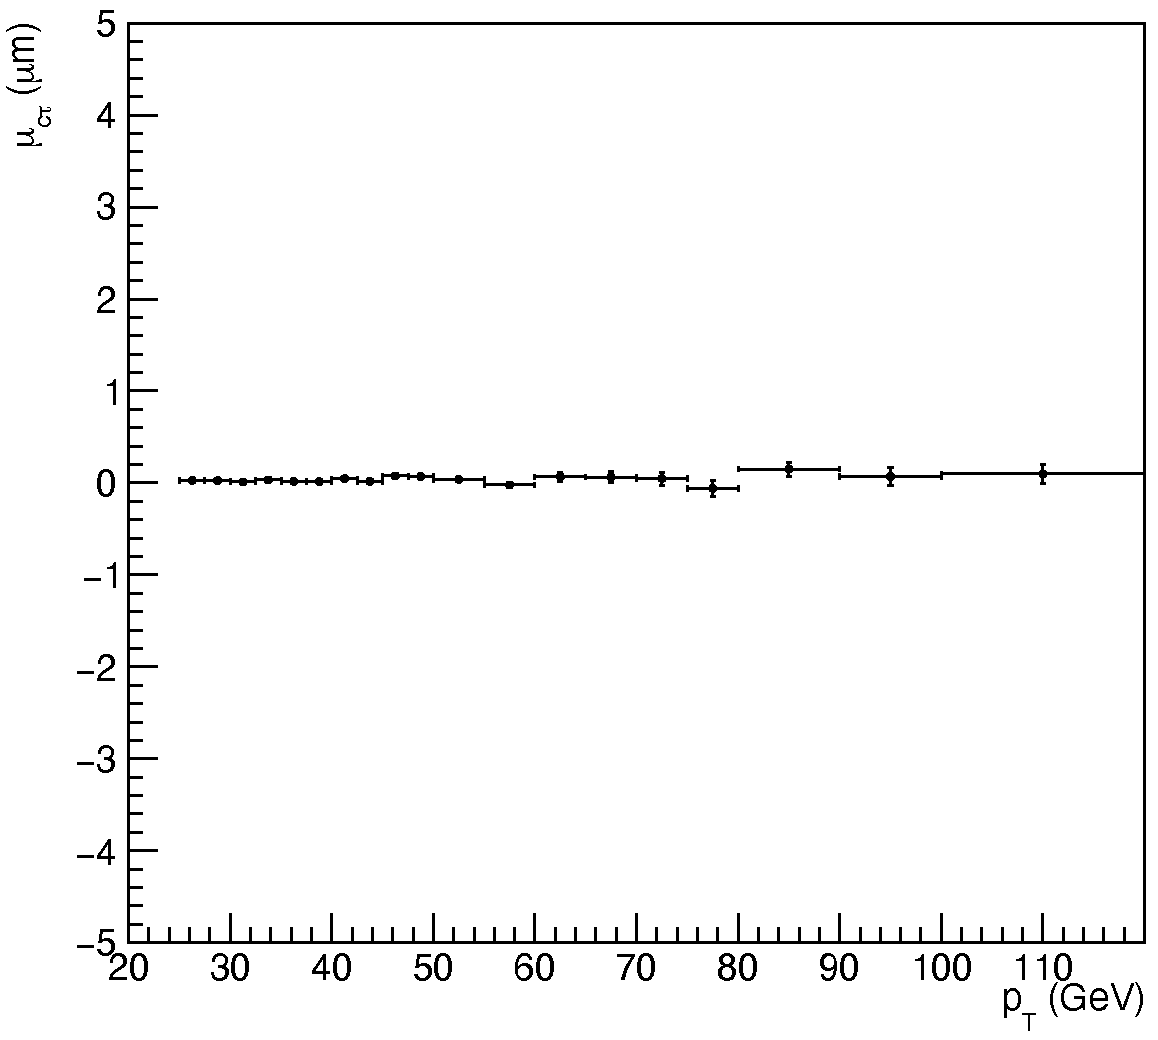
\includegraphics[width=0.45\textwidth]{Figures/chapter4/parf_mu.pdf}
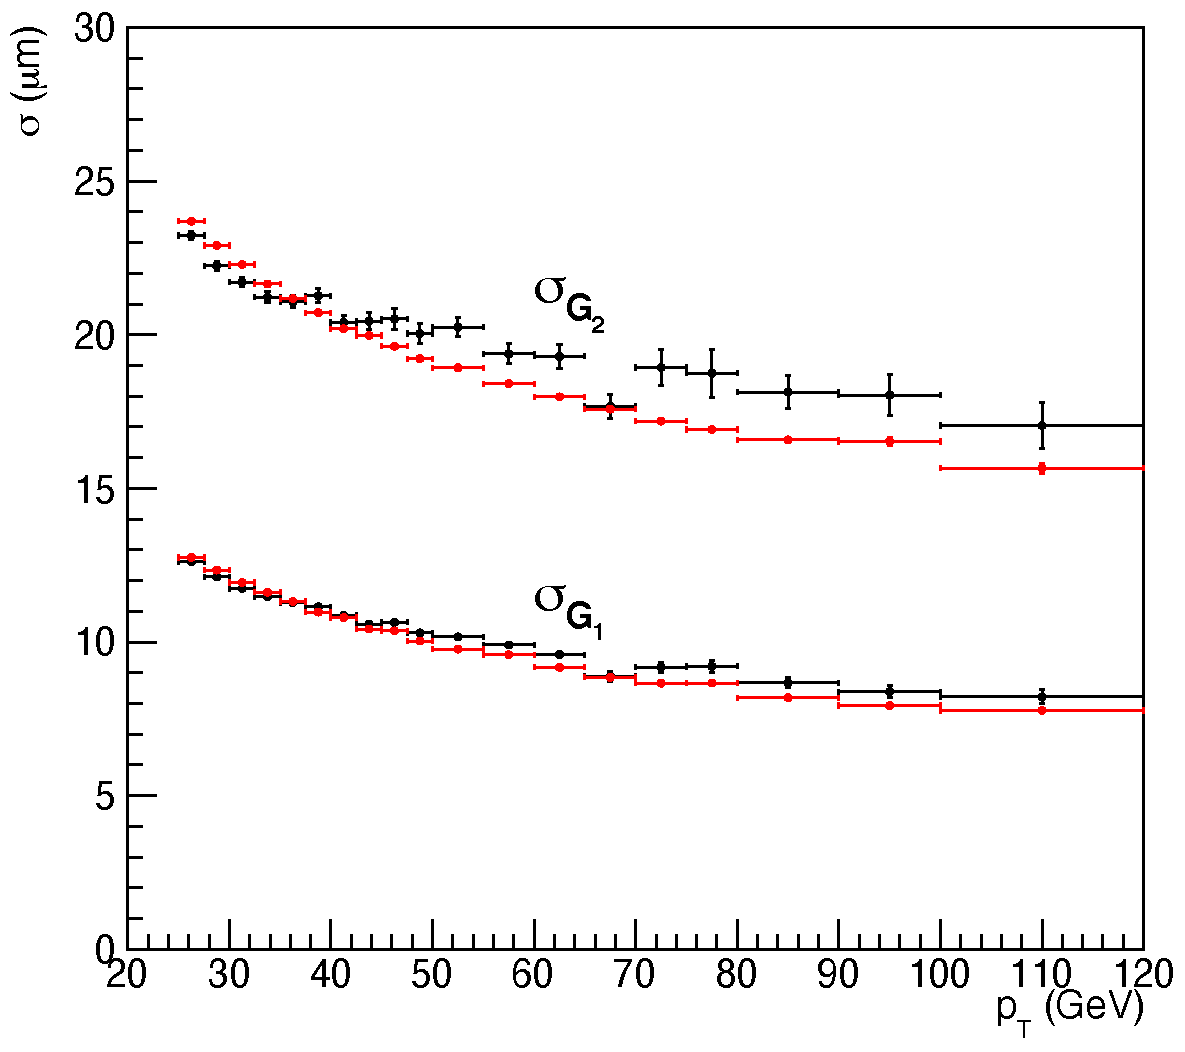
\includegraphics[width=0.45\textwidth]{Figures/chapter4/parB_sig1.pdf}
\caption{Left: \jpsi $\mu_{c\tau}$ vs.\ \pt when all shape parameters are left free.
Right: \jpsi $\sigma_{G_1}$ and $\sigma_{G_2}$ vs.\ \pt, 
before (black) and after (red) imposing that 
the $\mu_{c\tau}$ and $f_{G_1}$ parameters are independent of \pt.}
\label{fig:lt_sigmas}
\end{figure}

As we did for the definition of the  dimuon mass fit model,
we started by performing a series of preliminary studies,
including the option of independently fitting 
each of the 19 lifetime distributions, 
in the region $[-50,500]$~$\mu$m, 
with all the shape parameters free.
As expected, we see that this option leads to a fit with too much freedom,
as shown by the correlated fluctuations of the parameters 
$f_{G_1}$, $\sigma_{G_1}$ and $\sigma_{G_2}$.
We also see that $\mu_{c\tau}$ is clearly independent of \pt,
as shown in Fig.~\ref{fig:lt_sigmas}-left.
So, we proceed with a simultaneous fit of the 19 distributions 
imposing that the $\mu_{c\tau}$ and $f_{G_1}$ parameters are
independent of \pt.
The resulting $\sigma_{G_1}$ and $\sigma_{G_2}$ values show a 
much smoother variation with \pt, as shown in Fig.~\ref{fig:lt_sigmas}-right.

\vfill\newpage

The inverse slope of the \jpsi NP exponential function, $t_{\rm NP}$,
is essentially the same in both fitting options, 
as we can easily see in Fig.~\ref{fig:lt_slope}.
This is the most important shape parameter of the dimuon lifetime fits,
for the purpose of our analysis, given that all we need from these fits is
the fraction $f_{\rm NP}$, versus \pt.

\begin{figure}[h]
\centering
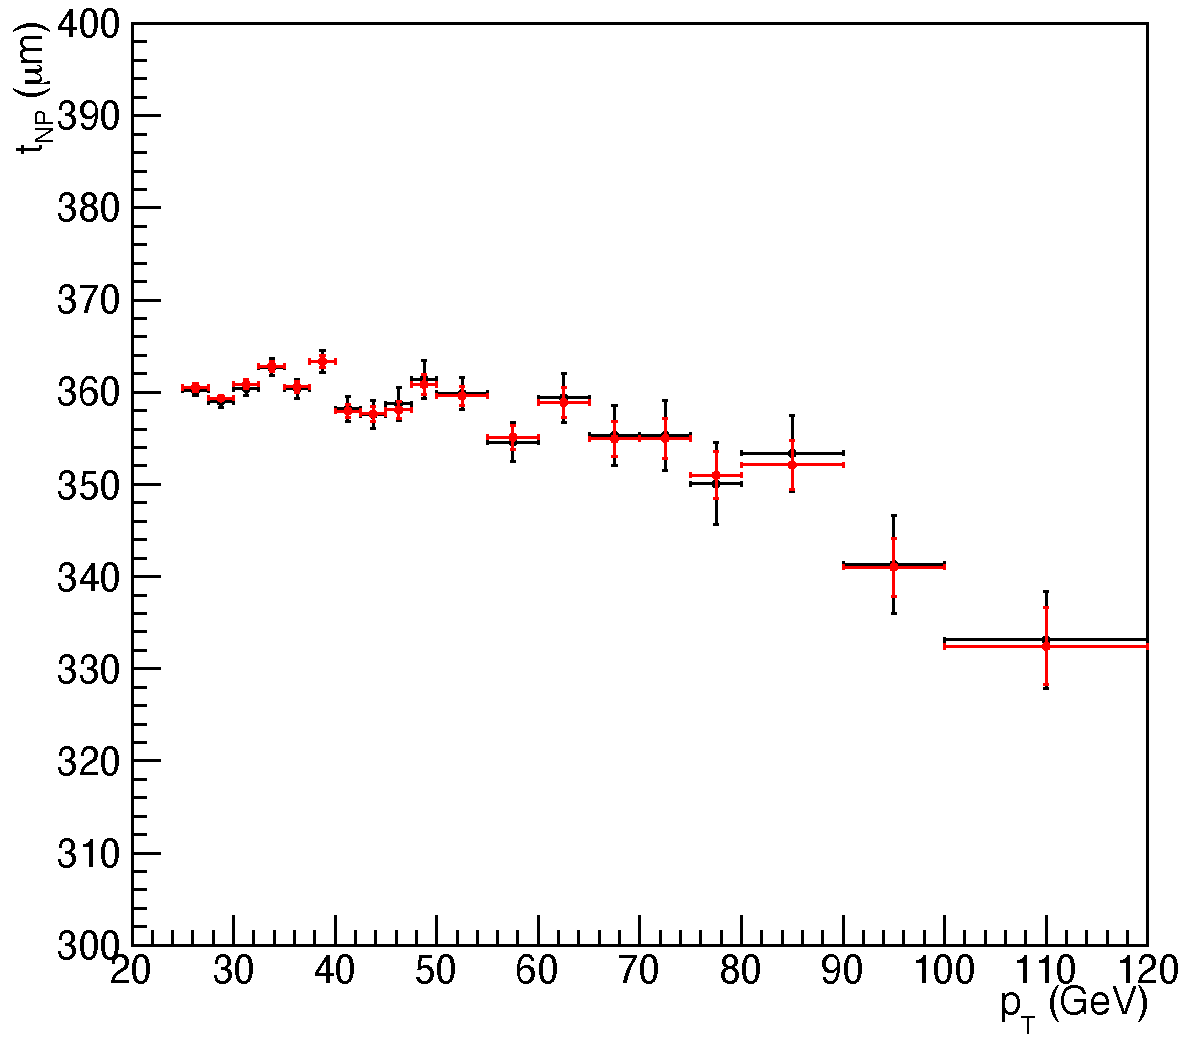
\includegraphics[width=0.45\textwidth]{Figures/chapter4/parB_lambda.pdf}
\caption{The inverse slope of the NP exponential function, $t_{\rm NP}$,
as a function of \pt, 
when the $\mu_{c\tau}$ and $f_{G_1}$ parameters are left free (black)
or are constrained to be independent of \pt (red).}
\label{fig:lt_slope}
\end{figure}

The analogous plots for the \psip case are shown in Fig.~\ref{fig:lt-psip}.

\begin{figure}[h]
\centering
\includegraphics[width=0.45\textwidth]{Figures/chapter4/parB_sig1-psip.pdf}
\includegraphics[width=0.45\textwidth]{Figures/chapter4/parB_lambda-psip.pdf}
\caption{Left: \psip $\sigma_{G_1}$ and $\sigma_{G_2}$ vs.\ \pt, 
before (black) and after (red) imposing that 
the $\mu_{c\tau}$ and $f_{G_1}$ parameters are independent of \pt.
Right: The inverse slope of the \psip NP exponential function, 
$t_{\rm NP}$, as a function of \pt, 
when the $\mu_{c\tau}$ and $f_{G_1}$ parameters are left free (black)
or are constrained to be independent of \pt (red).}
\label{fig:lt-psip}
\end{figure}

\vfill\newpage

The measured lifetime distributions are well described by the fit model;
there are no systematic trends in the pull distributions. 
Figures~\ref{fig:ctau-fits-psi} and~\ref{fig:ctau-fits-psip}
illustrate the fit quality in the \jpsi and \psip cases, respectively, 
for two typical \pt bins.

\begin{figure}[t]
\centering
\includegraphics[width=0.45\textwidth]{Figures/chapter4/ltfit_pt4.pdf}
\includegraphics[width=0.45\textwidth]{Figures/chapter4/ltfit_pt14.pdf}\\
\includegraphics[width=0.45\textwidth]{Figures/chapter4/ltpulls_pt4.pdf}
\includegraphics[width=0.45\textwidth]{Figures/chapter4/ltpulls_pt14.pdf}
\caption{Fitted \jpsi lifetime distributions for two \pt bins (top) 
and corresponding pull distributions (bottom).
The vertical black dashed lines mark the limits of the PR and NP regions. 
The total fit function is shown in blue, 
while the dash-dotted green and violet lines 
represent the PR and NP contributions, respectively.}
\label{fig:ctau-fits-psi}
\end{figure}

\begin{figure}[p!]
\centering
\includegraphics[width=0.45\textwidth]{Figures/chapter4/ltfit_psip_pt2.pdf}
\includegraphics[width=0.45\textwidth]{Figures/chapter4/ltfit_psip_pt5.pdf}\\
\includegraphics[width=0.45\textwidth]{Figures/chapter4/pulls_ltfit_psip_pt2.pdf}
\includegraphics[width=0.45\textwidth]{Figures/chapter4/pulls_ltfit_psip_pt5.pdf}
\caption{Fitted \psip lifetime distributions for two \pt bins (top) 
and corresponding pull distributions (bottom).
The vertical black dashed lines mark the limits of the PR and NP regions. 
The total fit function is shown in blue, 
while the dash-dotted green and violet lines 
represent the PR and NP contributions, respectively.}
\label{fig:ctau-fits-psip}
\end{figure}

\vfill\newpage

As mentioned earlier, the fraction of events in the prompt (``Peak") region 
that are due to \jpsi (or \psip) mesons produced in B decays, $f_{\rm NP}$, 
is evaluated (in each \pt bin) by integrating the fitted $L_{\rm NP}$ function
in that window and then dividing the result by the total number of Peak events.
The results are shown in Fig.~\ref{fig:fNP}, for the \jpsi and \psip analyses.
As expected from previous analyses,
the \jpsi ``non-prompt fraction" increases with \pt and then saturates.
The results are identical when the $\mu_{c\tau}$ and $f_{G_1}$ parameters
are left free (black points) or are common to all \pt bins (red points).

\begin{figure}[h]
\centering
\includegraphics[width=0.48\textwidth]{Figures/chapter4/fNP-jpsi.pdf}
\includegraphics[width=0.48\textwidth]{Figures/chapter4/fNP-psip.pdf}
\caption{Measured $f_{\rm NP}$ fractions vs.\ \pt, 
for the \jpsi (left) and \psip (right) analyses.}
\label{fig:fNP}
\end{figure}

Knowing the fractions of non-prompt \jpsi (or \psip) mesons 
and continuum muon pairs in the Peak region, 
we can deduce the corresponding fraction of prompt \jpsi (or \psip) mesons.
The results are shown in Fig.~\ref{fig:fractions}, for the \jpsi and \psip analyses.

\begin{figure}[h]
\centering
\includegraphics[width=0.48\textwidth]{Figures/chapter4/f_comp_corr-jpsi.pdf}
\includegraphics[width=0.48\textwidth]{Figures/chapter4/f_comp_corr-psip.pdf}
\caption{Fractional contributions from each of the three sources of dimuons
in the prompt region of the \jpsi (left) and \psip (right) events.}
\label{fig:fractions}
\end{figure}

\vfill\newpage

\subsection{An interesting side remark}

We conclude this chapter with an interesting side remark:
the \emph{shape} of the \pt dependence of the background contamination functions 
can be determined without any fits.
Indeed, it is sufficient to compute the ratios between the event yields 
counted in the NP or mass sideband regions and the Peak region.
Figure~\ref{fig:fractions_from_yields} shows, using the \jpsi example, that 
this trivial alternative procedure gives virtually the same trends vs.\ \pt.

\begin{figure}[h]
\centering
\includegraphics[width=0.48\textwidth]{Figures/chapter4/fitcomp_fSB.pdf}
\includegraphics[width=0.48\textwidth]{Figures/chapter4/fitcomp_fNP.pdf}
\caption{Comparison between the fitted background fractions,
$f_{\rm Bg}$ (left) and $f_{\rm NP}$ (right),
with the corresponding ratios of counts, for the \jpsi events.}
\label{fig:fractions_from_yields}
\end{figure}
